\chapter{関連研究と諸概念の整理}
\label{chap:prevresearch}

\section{ユーザビリティ}

英単語としてのusabilityはuse(使う)+able(できる)+ity(こと)から構成されており,「使うのに便利で実用的な」という意味で14世紀から使われていた\cite{oed:usability}\cite{kurosu}.しかし,概念としてのユーザビリティがアカデミアで取り上げられるようになったきっかけはコンピュータの登場と普及だった\cite{kurosu}.コンピュータはトレーニングを受けた専門家が使用するものとして作られたが,一般への普及が図られるなかで使いやすさを検討する必要性が出てきたのだと考えられる.

Shackelによると彼以前にMirrorやBennetがユーザビリティに言及しているが,彼らはユーザビリティを「使いやすさ(ease of use)」とほぼ同義として扱っていた\cite{shackel1991human}\cite{kurosu}.Nielsenは,ユーザビリティを複数の要素の上位概念であるとし,下位概念として学習可能性(Learnabiliity),Efficiency(効率性),Memorability(記憶のしやすさ),Errors(エラー),Satisfication(満足度)を挙げている\cite{nielsen1994}. 

国際規格としてユーザビリティが定義されたのはISO9241シリーズ「人間とシステムの相互作用の人間工学(Ergonomics of Human-System Interaction)」であり,ISO9241-11:1998ではユーザビリティを「特定のユーザーが,特定の使用状況において,特定の目標を達成するために,製品を有効,効率的かつ満足に使用できる度合い.(Extent to which a product can be used by specified usersto achieve specified goals witheffectiveness, efficiency and satisfaction in a specified context of use.)」と定義している.
%引用
この定義はISOの関係者やベヴァンらが普及活動に力を入れた結果標準としての地位を獲得するにいたった\cite{kurosu}.この定義は現在でも一般の技術者に浸透していると考えられる.しかし黒須は,客観的に計測可能な有効性や効率性と主観的なものである満足性を同列に扱うことについて疑問を呈しており,有効かつ効率的であれば満足性が上がるため,満足性はより上位の概念であると主張している\cite{kurosu}.

ISO/IEC9126-1:2001やISO/IEC25010:2011 SQuaRE(System and Software Quality Requirements and Evaluation)では体系化が進められており,ユーザビリティが品質モデルの一部に組み込まれた形となっている.SQuaRE
%引用
では,図\ref{fig:square}のように品質モデルが製品品質モデルと利用時の品質モデルに分けられており,ユーザビリティは製品品質の下位概念に位置づけられている.そして,有効性,効率性,満足性は利用時の品質の中に置かれている.

\begin{figure}[htbp]
  \begin{minipage}{\hsize}
    \begin{center}
       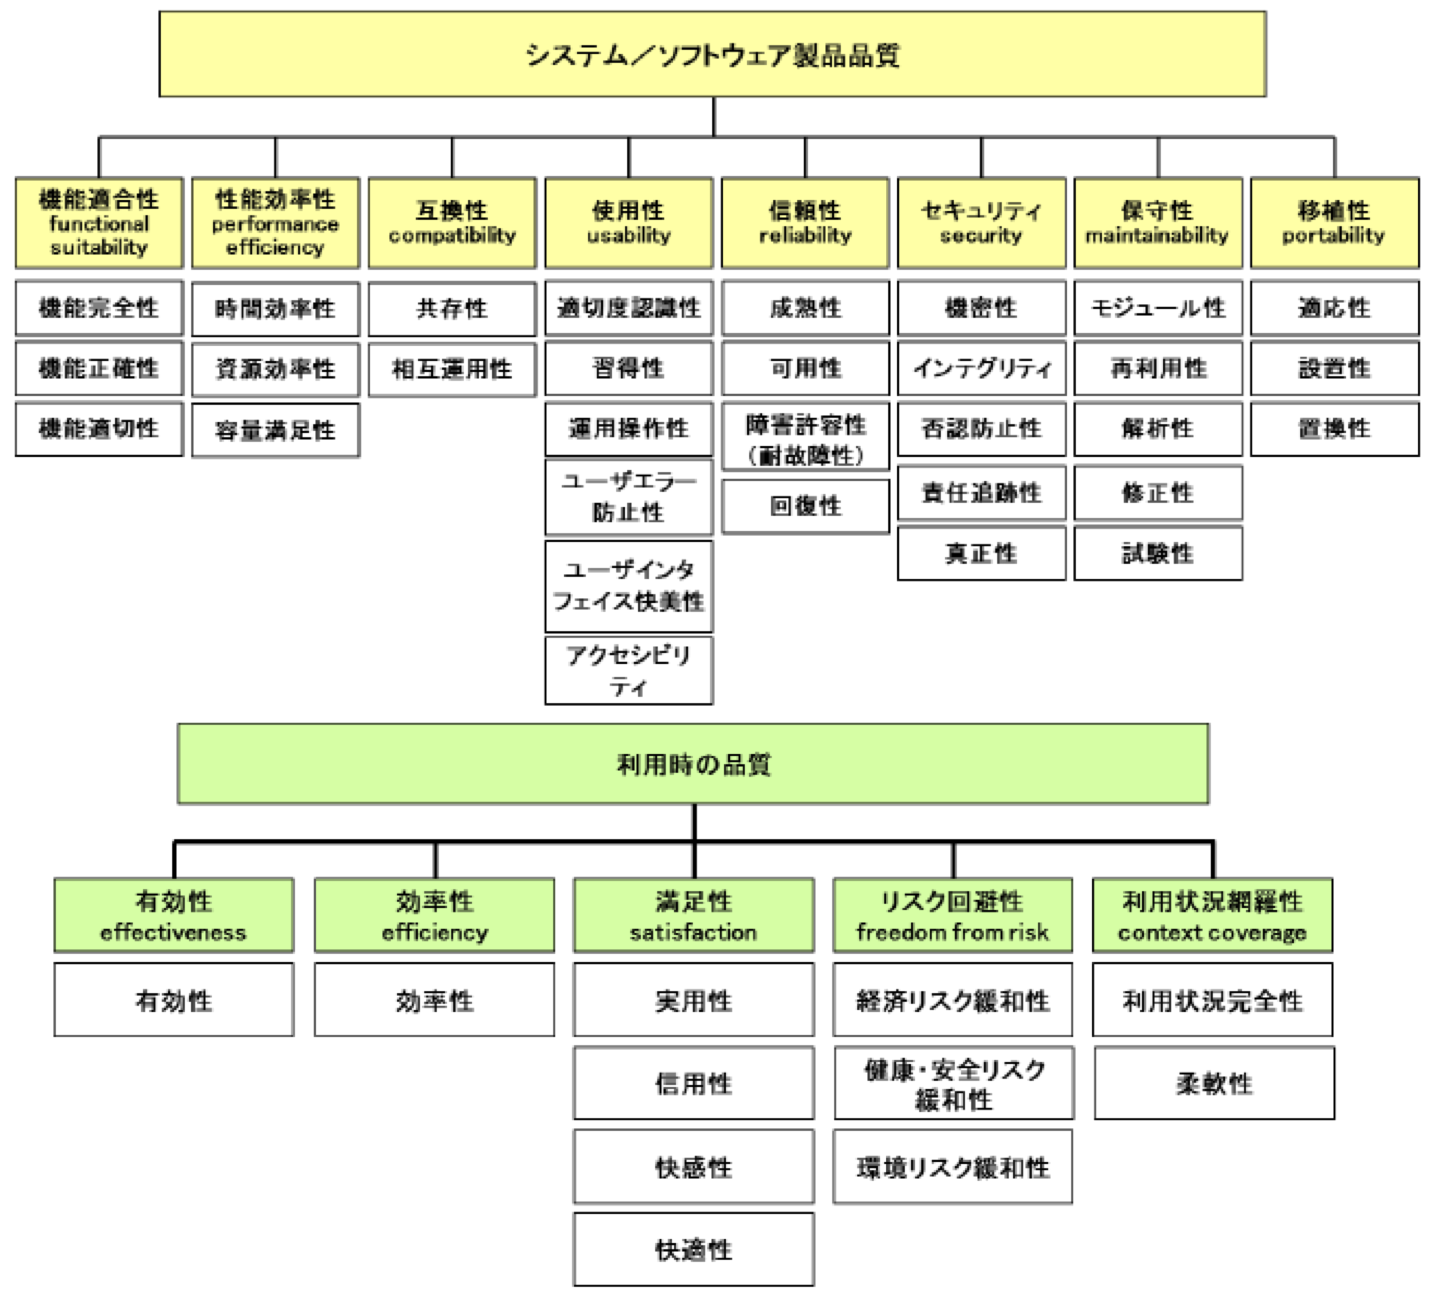
\includegraphics[width=100mm]{img/square.png}
    \end{center}
    \caption{SQuaREを基にしたJIS X 25010:2013の品質モデル}
    \label{fig:square}
  \end{minipage}
\end{figure}

SQuaREの改訂では
%引用
,設計上の品質である製品品質とユーザが使用した際のユーザにとっての品質である利用時の品質とに分けた点が重要である.人間の思い通り予想通りに動いてくれるシステムを設計しようとする人間中心設計\cite{kurosu2013}の考え方の普及などにより,設計時にユーザの存在をこれまで以上に重要視する動きの中でユーザの利用時に特に注目する必要が出てきたと考えられる.この考え方は後述のUXの概念に関わっており,一方でユーザビリティはユーザに目を向けたものではなく製品設計レベルの概念だということになる.

本研究では,ユーザがシステム利用時にどのような生理的反応を見せるかということに注目 しており,SQuaREの定義でいうところの利用時の品質やその下位概念の満足性を測定することを目指しているといえる.第\ref{chap:introduction}章では,Nielsenのヒューリスティック評価はユーザや利用シーンの多様性を考慮しておらず不十分であると述べた.確かにニールセン自身が定義したユーザビリティには満足度が含まれていたためにユーザによってユーザビリティが異なることが考えられた.しかしSQuaREの定義では,ユーザビリティは実ユーザの存在から離れ特定ユーザ・特定の使用状況・特定の目的において満たされていればよく,Nielsenのヒューリスティック評価が有効になると考えられる.一方,本研究で扱うユーザテストでは,多様なユーザに目が向けられており,SQuaREの定義におけるユーザビリティという概念は当てはめることができない.そこで,SQuaREの利用時の品質などの概念を拡張した概念であるUXについて検討する.なお,本論文ではユーザビリティという用語は基本的に使用せず,使用する場合は「使いやすさ」という一般的な意味でのみ使用する.

\section{UX}

User Experienceという言葉は,1995年にはAppleのヒューマンインタラクショングループで使われており\cite{norman1995},ヒューマンインタフェースやユーザビリティといった言葉ではカバーできない工業デザインのグラフィック,インタフェース,物理的なインタラクション,マニュアルなど人がシステムを利用する際のあらゆる側面を含む言葉として発明したとNormanがインタビューで述べている\cite{normaninterview}.しかしその後,UXという言葉の普及に伴ってあらゆる事象に使われるようになり本来の意味が不明瞭になりつつあった.そこでロトらによってUX白書でUXの定義が定められた.UX白書では,UXとは``「一般的な意味における経験」とは異なり,システムと出会うことにおける経験''であるとしている\cite{uxwhitepaper}.

UX白書によるUXの定義には「システムと出会うこと」という文言が含まれている.つまり,UXは製品の設計やシステム自体についての概念ではなくユーザと製品との間に生まれるものであり,前述のSQuaREの利用時品質に関連が深いことがわかる.また,UX白書ではUXに影響する要素(factor)として,ユーザとシステムに加えて文脈を挙げている\cite{uxwhitepaper}.UXはこれらの3つの掛け合わせで表現されるものでどれかが変化すればUXも変化するといえる.

UXは製品が最終的にユーザにどのように受け取られるかという重要な概念ではあるが,一方で製品設計においては「UXを向上させる」ということが必ずしも正しいとは限らない.UXはシステムに対してユーザの数×文脈の数だけ存在するためそれら全てを向上させることは不可能だからである.実ユーザのUXを考慮して,ビジネス上の目標あるいは技術上の制約に沿うように製品設計に落とし込み,その上で製品品質を向上させる必要がある.

\subsection{満足性}

黒須の品質特性図(図\ref{fig:kurosu2015})にあるように,UXはSQuaREの利用時品質に対応しており,それには客観的利用品質と主観的利用品質が含まれる.客観的利用品質は測定可能な指標であり既に評価手法の研究は十分なされているため本研究では取り上げない.
%いくつか引用
また,客観的利用品質は主観的利用品質の原因であり,主観的利用品質は客観的利用品質の要素を知覚した結果が含まれたものであると見ることができる.そのため主観的利用品質と客観的利用品質の接続が重要になる.

主観的利用品質には,達成感,安心感,楽しさ,喜ばしさ,嬉しさなどの感情が含まれており,これらと従属関係を持ち最高位に位置する言葉として満足が挙げられている\cite{kurosu2011}.つまり,満足性を測定することで主観的利用品質を評価することができ,知覚という形で客観的利用品質も満足性の度合いに含まれるためUX全体を評価することに繋がる可能性がある.このように,何らかの指標によって満足性を測定することがUXを評価するうえで重要である.

\subsection{時間相}

ISOのSQuaREに対してUX白書のUXの定義では時間相が明確になっている.どれくらいの期間に焦点を当てるかという視点で分類すると一時的UX,エピソード的UX,累積的UXに分けられる.また,これに使用前の期待などを指す予期的UXを含め図\ref{fig:lifecycle}のようにライフサイクルとして捉えることもできる\cite{uxwhitepaper}.

\begin{description}
   \item[一時的UX]システム使用中の特定のインタラクションに対する感情の変化
   \item[エピソード的UX]利用エピソードに関する評価
   \item[累積的UX]システムをしばらく使用し利用中や利用していない時間を通して形成される評価
\end{description}

\begin{figure}[htbp]
  \begin{minipage}{\hsize}
    \begin{center}
       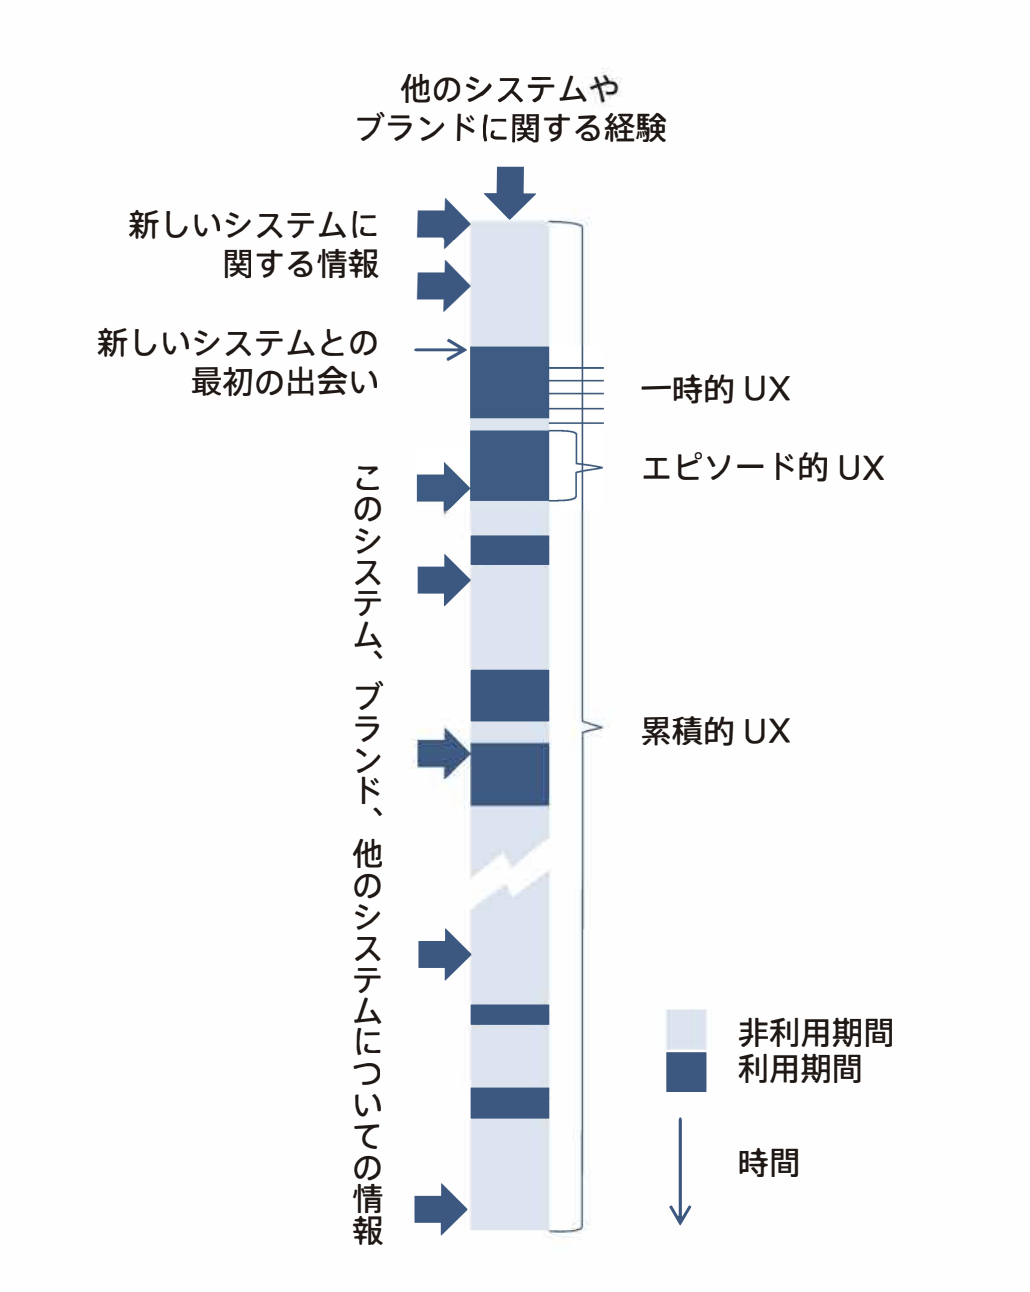
\includegraphics[width=100mm]{img/lifecycle.png}
    \end{center}
    \caption{UXのライフサイクル\cite{uxwhitepaper}}
    \label{fig:lifecycle}
  \end{minipage}
\end{figure}

UXの変化を時系列で捉えるための方法として黒須がUXグラフ\cite{kurosu2015}を提唱している.これは,入手前の期待,入手時の感情などを含めて製品を使用した際のあるいは使用していないときの出来事とその満足度レベルを列挙したうえで,縦軸に満足度レベル,横軸に時間をとってグラフ化するものである.これはユーザ自身に記入させるものでユーザにとってのUX変化が累積的UXのレベルで可視化することができる.一方,エピソード的UXの中で,個別のインタラクションに対する一時的UXまではユーザに思い出しながら書いてもらうことが困難であり全て書き切れるとは言えない.また,評価対象は満足度という主観的なものではあるものの,ユーザに自己申告させる方式では正しく評価できない可能性を排除できない.つまり主観的評価と客観的評価の双方に着目した指標が必要である.

\section{UXメトリクス}

UXメトリクスとは,UXを何らかの数的指標として測定するものであり,UXを製品設計に活用するためには欠かせない手法である.UXメトリクスには,パフォーマンスメトリクスや自己申告メトリクス,行動・生理メトリクスなどがあり\cite{tullis2014},これらを組み合わせて評価することが必要であると前に述べた.利用時の品質特性に当てはめると,パフォーマンスメトリクスは客観的利用品質の測定であり,自己申告メトリクスや行動・生理メトリクスは主観的利用品質の測定であるといえる.パフォーマンスメトリクスは有用であるものの,システムの全ての部分を評価することはできないため,問題がありそうな部分や変更を加えようとする一部分のみを切り出して測定することになる.自己申告メトリクスは質問紙や記述式アンケートに代表される手法であり,前述のUXグラフもその一例である.主観的利用品質つまり満足性を評価するもう一つの手法である行動・生理メトリクスは質問紙では把握しきれない細かな情報を生かすことができると期待される.

行動・生理メトリクスはユーザのあらゆる行動や生理反応を記録しようとするもので,様々な手法が研究されている.まず,システムを使用しているユーザを直接あるいはビデオで記録したものを観察し,言語行動や非言語行動を抽出することは一般的な方法である.
%引用
言語行動としては,システムを褒めたり否定したりする直接的なコメントに加えて,「どこを押せばいいんですか?」などの質問などが考えられる.非言語行動としては,顔の表情や集中力,いらだち,眼を細めて読もうとするなどの行動から読み取ることができる.このような方法は特別なシステムが必要なくいつでも始められる一方で観察者の能力によって読み取る情報の精度にばらつきが出ることが考えられる.

\subsection{センサを用いた生理メトリクスの測定}

観察するための機器が必要な指標としては,顔の表情,アイトラッキング,瞳孔の直径,ストレス\cite{tullis2014}などがある.

顔の表情は直接観察することもできるが,システムを使うことで自動的にかつ取りこぼしなく計測しようとする研究がなされている.Hazlettらは2007年に顔面筋電位を用いて表情を分類する研究を行っている\cite{faceemg}.現在であれば表情をビデオで収録し機械学習によって分類すれば筋電位センサのような大がかりな装置を装着することなく表情を分析することが可能であると考えられる.Staianoらはシステム使用時の映像に対しインタラクション毎に表情の注釈をつけるシステムを提案しており,映像の表情分類には機械学習を使用している\cite{uxmate}.

アイトラッキングはtobii社がtobiipro\cite{tobii}というアイトラッカー及びその分析ツールを発売している.事前のキャリブレーションが必要なほか,機器が高額であるため通常のシステム開発で活用されているとは言えないがUX評価での実績はある.
%引用
アイトラッキングで行える分析には特定の要素やエリアを見たユーザの割合,特定の要素やエリアを見た時間,特定の要素に気づくまでに要した時間,眼の動きの距離,注視の時間などがある\cite{tullis2014}.瞳孔の直径についての情報は多くのアイトラッカーで得ることができる.瞳孔反応は明るさのレベルに反応する以外に認知処理や興奮,興味の高まりに相関することがわかってる.しかし,瞳孔反応は様々な心理状態に反応するためその理由が肯定的なのか否定的なのかを分類することが難しいと言われている\cite{tullis2014}.

ストレスの測定は満足性に密接に関係すると考えられ,様々な手法が検討されている.本研究で扱う容積脈波もストレスの測定の一種であるといえる.他の様々なストレス評価手法については後述する.

\subsection{ストレスの測定}

ストレスの測定とは,ストレスと相関があるとされている生理反応を測定しその度合いでストレスを判断するもので,様々なセンサとそれを用いた指標が提案されている.

皮膚伝導率(GSR: Galvanic Skin Response)はストレスが上がり発汗量が増えることで皮膚の電気抵抗が変化することを用いたもので,タスクパフォーマンスとの相関が明らかになっている\cite{lin2005}.皮膚伝導率計は手に装着するため自由な指の動きや手での操作を阻害しユーザビリティ評価に使うことができなかった.そこで,手のひらの一部分のみを覆い,指の動きを阻害しない皮膚伝導率計であるGalvactivator\cite{galvactivator} が提案されている.しかし,ユーザビリティを評価するうえで少しであっても手に異物を装着することは避けるべきと考えられる.

心拍数変動(HRV: Heart Rate Variability)は心電図(ECG:Electrocardiogram)を用いて測定するものでストレスと関連があることが知られている.これをユーザビリティ評価に活用する研究は古くから行われており,Roweらの研究では心拍数(HR: Heart Rate)の変化が目標処理能力の低下する時点を示す可能性を指摘している\cite{hrv1998}.光電式容積脈波記録(PPG: Photoplethysmography)を用いて計測する脈拍変動(PRV: Pulse Rate Variability)でも心拍変動と同様の結果が得られることがわかっている\cite{ppg}.医療機関や研究機関ではECGの使用が可能であるが,機器が大がかりになるため通常の開発では使用することができなかった.そこで最近ではApple Watchなどのスマートウォッチにも搭載され日常的に使用が可能な光電式容積脈波を用いた手法に期待できる.

脳波記録(EEG: Electroencephalography)は脳の電気信号を脳波計によって記録するもので,様々な刺激に対して反応することが知られている.Amaralらの研究では簡単とラベリングされたタスクと難しいとラベリングされたタスクについてF,C,P,O領域の8つの電極から得られた7つの周波数帯の平均パワースペクトル密度を特徴量としてサポートベクターマシン分類器で評価したところ有意な差が見られたとしている\cite{eeg}.

ストレス評価には.これらの他にも様々な手法が検討されているが,一般的なユーザビリティ評価でストレスを測定することはほとんど無い.ストレスの評価に使用する機器が大がかりであったり高価であったりするうえ,センサを装着すること自体が被験者のストレスになり正常な測定ができなくなる可能性があるからである\cite{tullis2014}.しかし,容易に計測できるようになればシステムの主観的品質・満足性を他の方法に対して比較的ダイレクトに近い情報を取りこぼしなく得られる可能性がある.

\section{容積脈波(BVP)}

光電式容積脈波(PPG)は血中のヘモグロビンが吸収する波長の光を照射し反射光や透過光の変化からヘモグロビン量を測る手法である\cite{pulseoximeter}.脳波(ECG)と比較して装置が小型かつ使用が容易であり,脳波や皮膚伝導率(GSR)のような使用時の違和感が少ないことが特徴である.実際の装置を図\ref{fig:device2}と図\ref{fig:device1}に示す.図\ref{fig:device2}は指先に装着するカフ式のものであり,中央のクリップを人差し指に装着する.図\ref{fig:device1}は耳朶に装着するもので黒い部分が耳朶に装着するクリップになっており,右下に移っている本体はBluetoothでコンピュータに接続する.耳朶用を使用すればシステムの操作時に邪魔にならない.

\begin{figure}[htbp]
\begin{minipage}{0.5\hsize}
    \begin{center}
       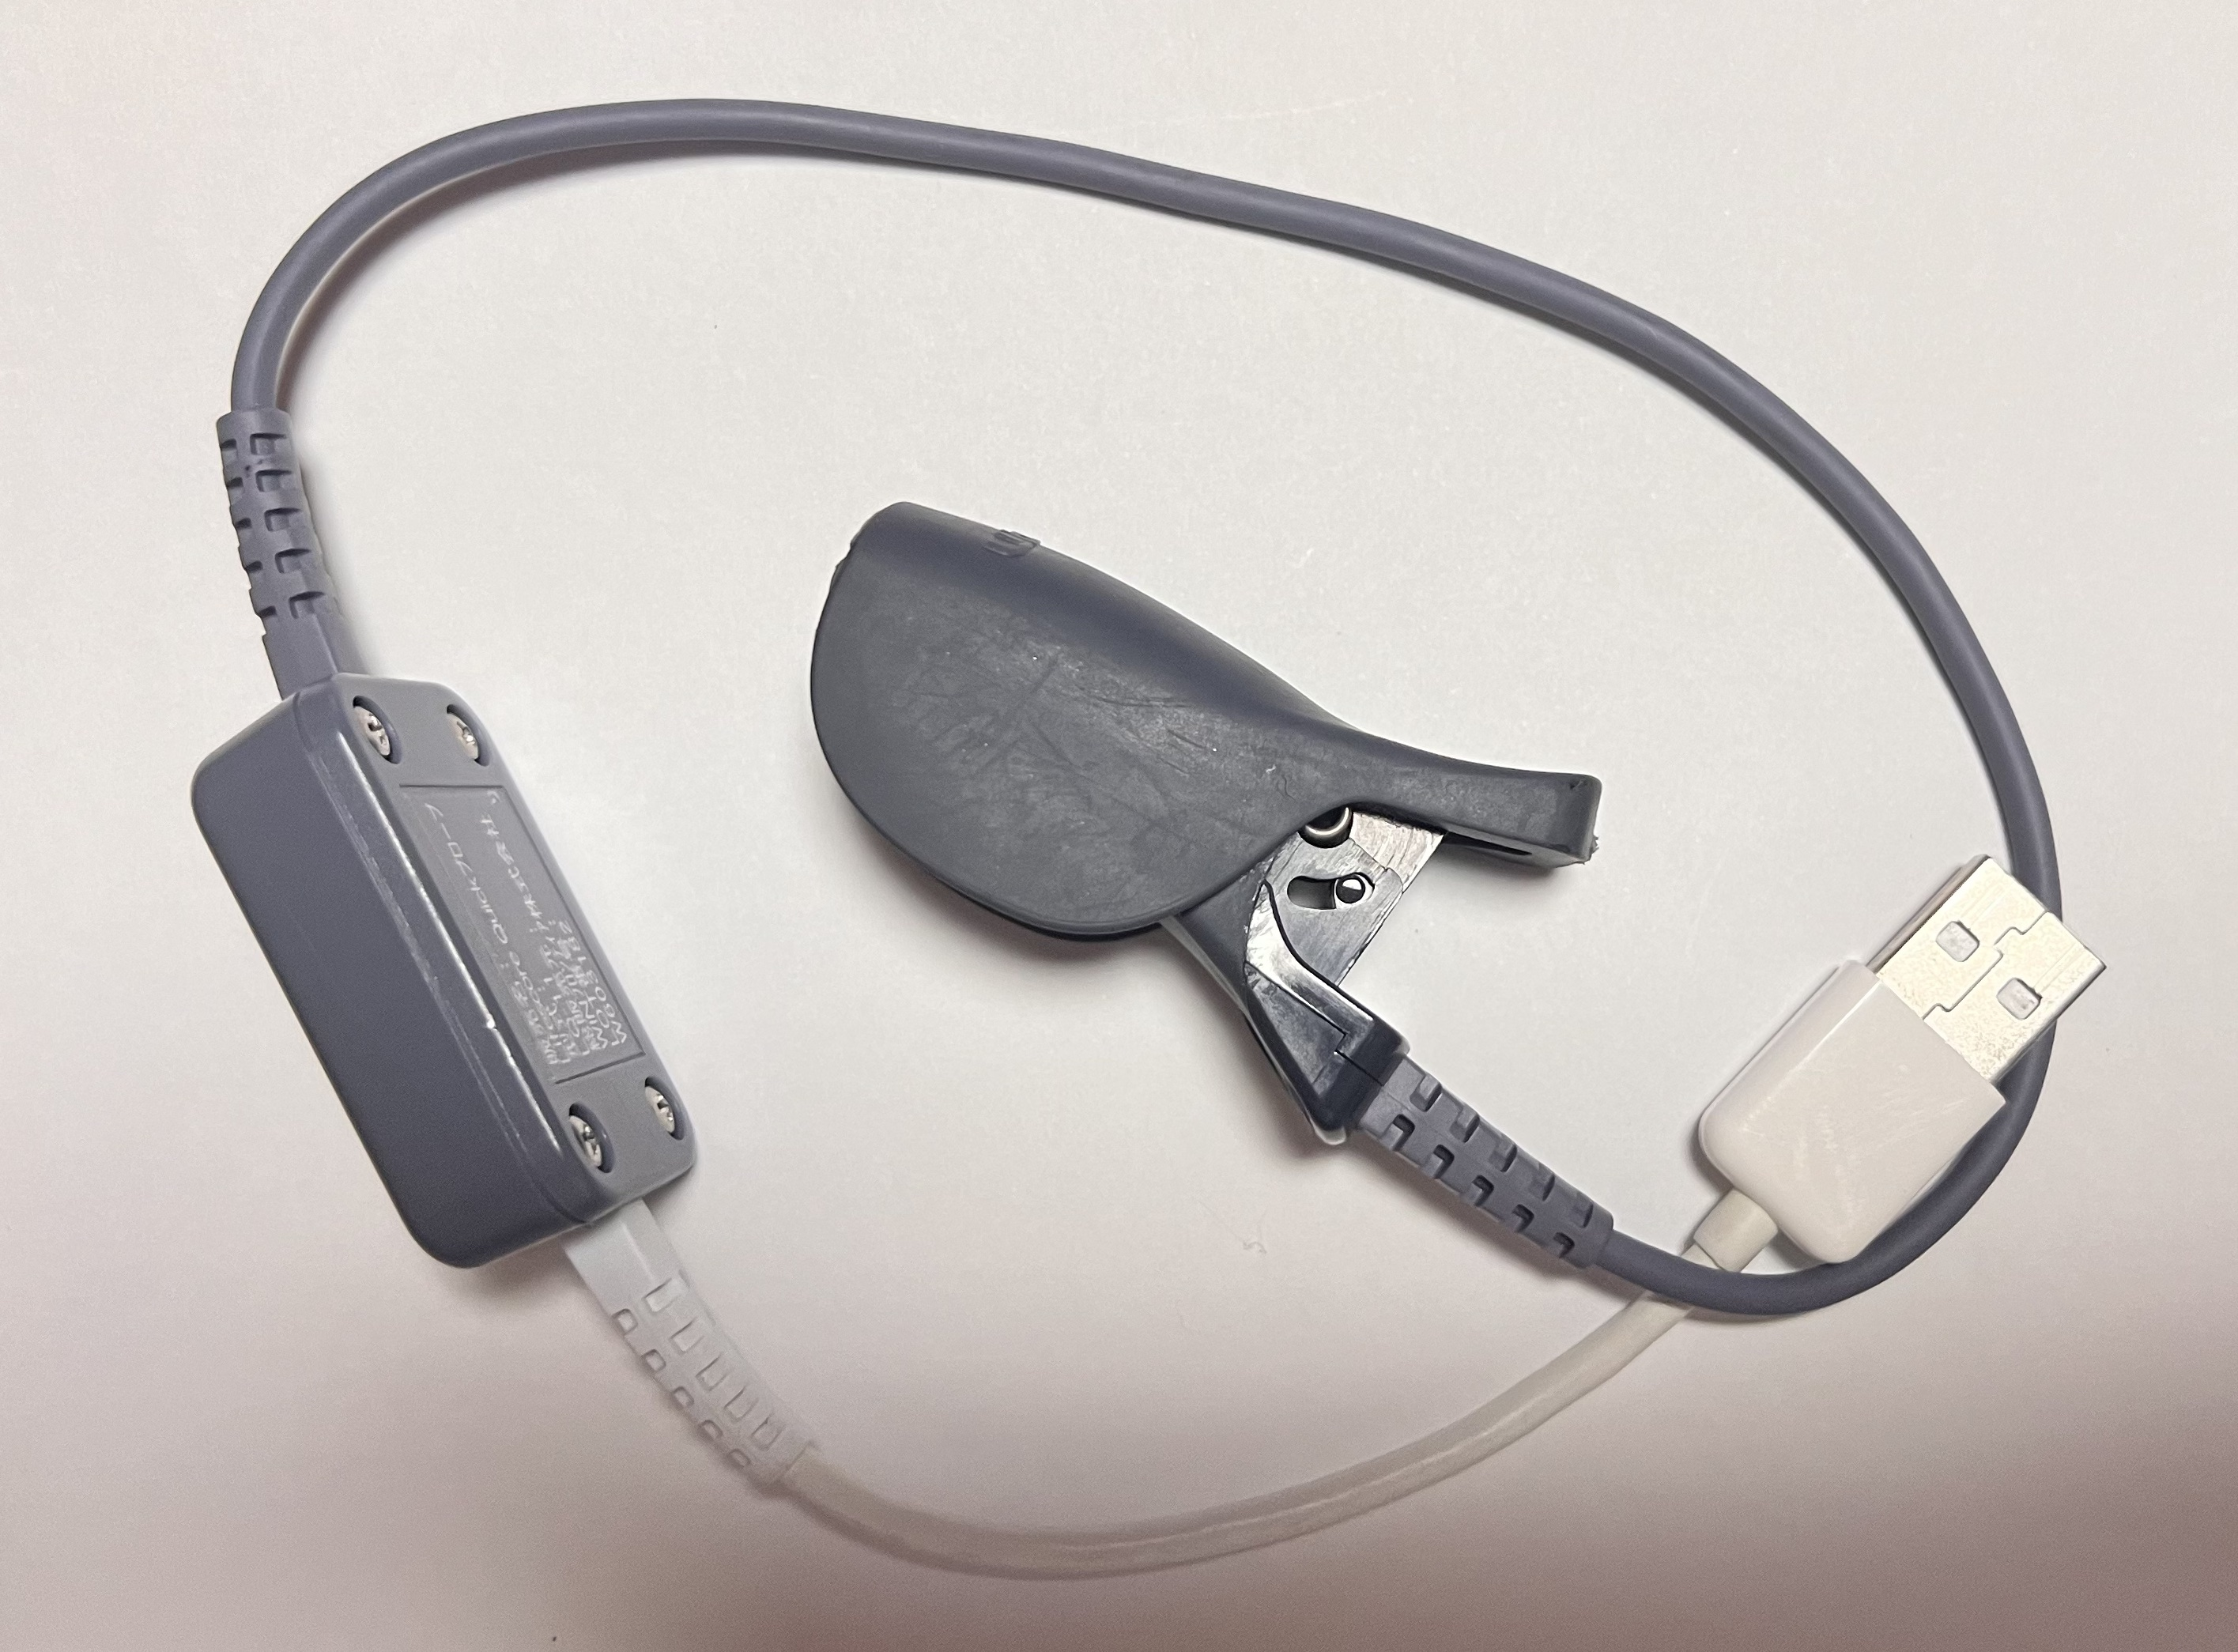
\includegraphics[width=60mm]{img/device2.jpg}
    \end{center}
    \caption{指尖用光電式容積脈波計}
    \label{fig:device2}
  \end{minipage}
  \begin{minipage}{0.5\hsize}
    \begin{center}
       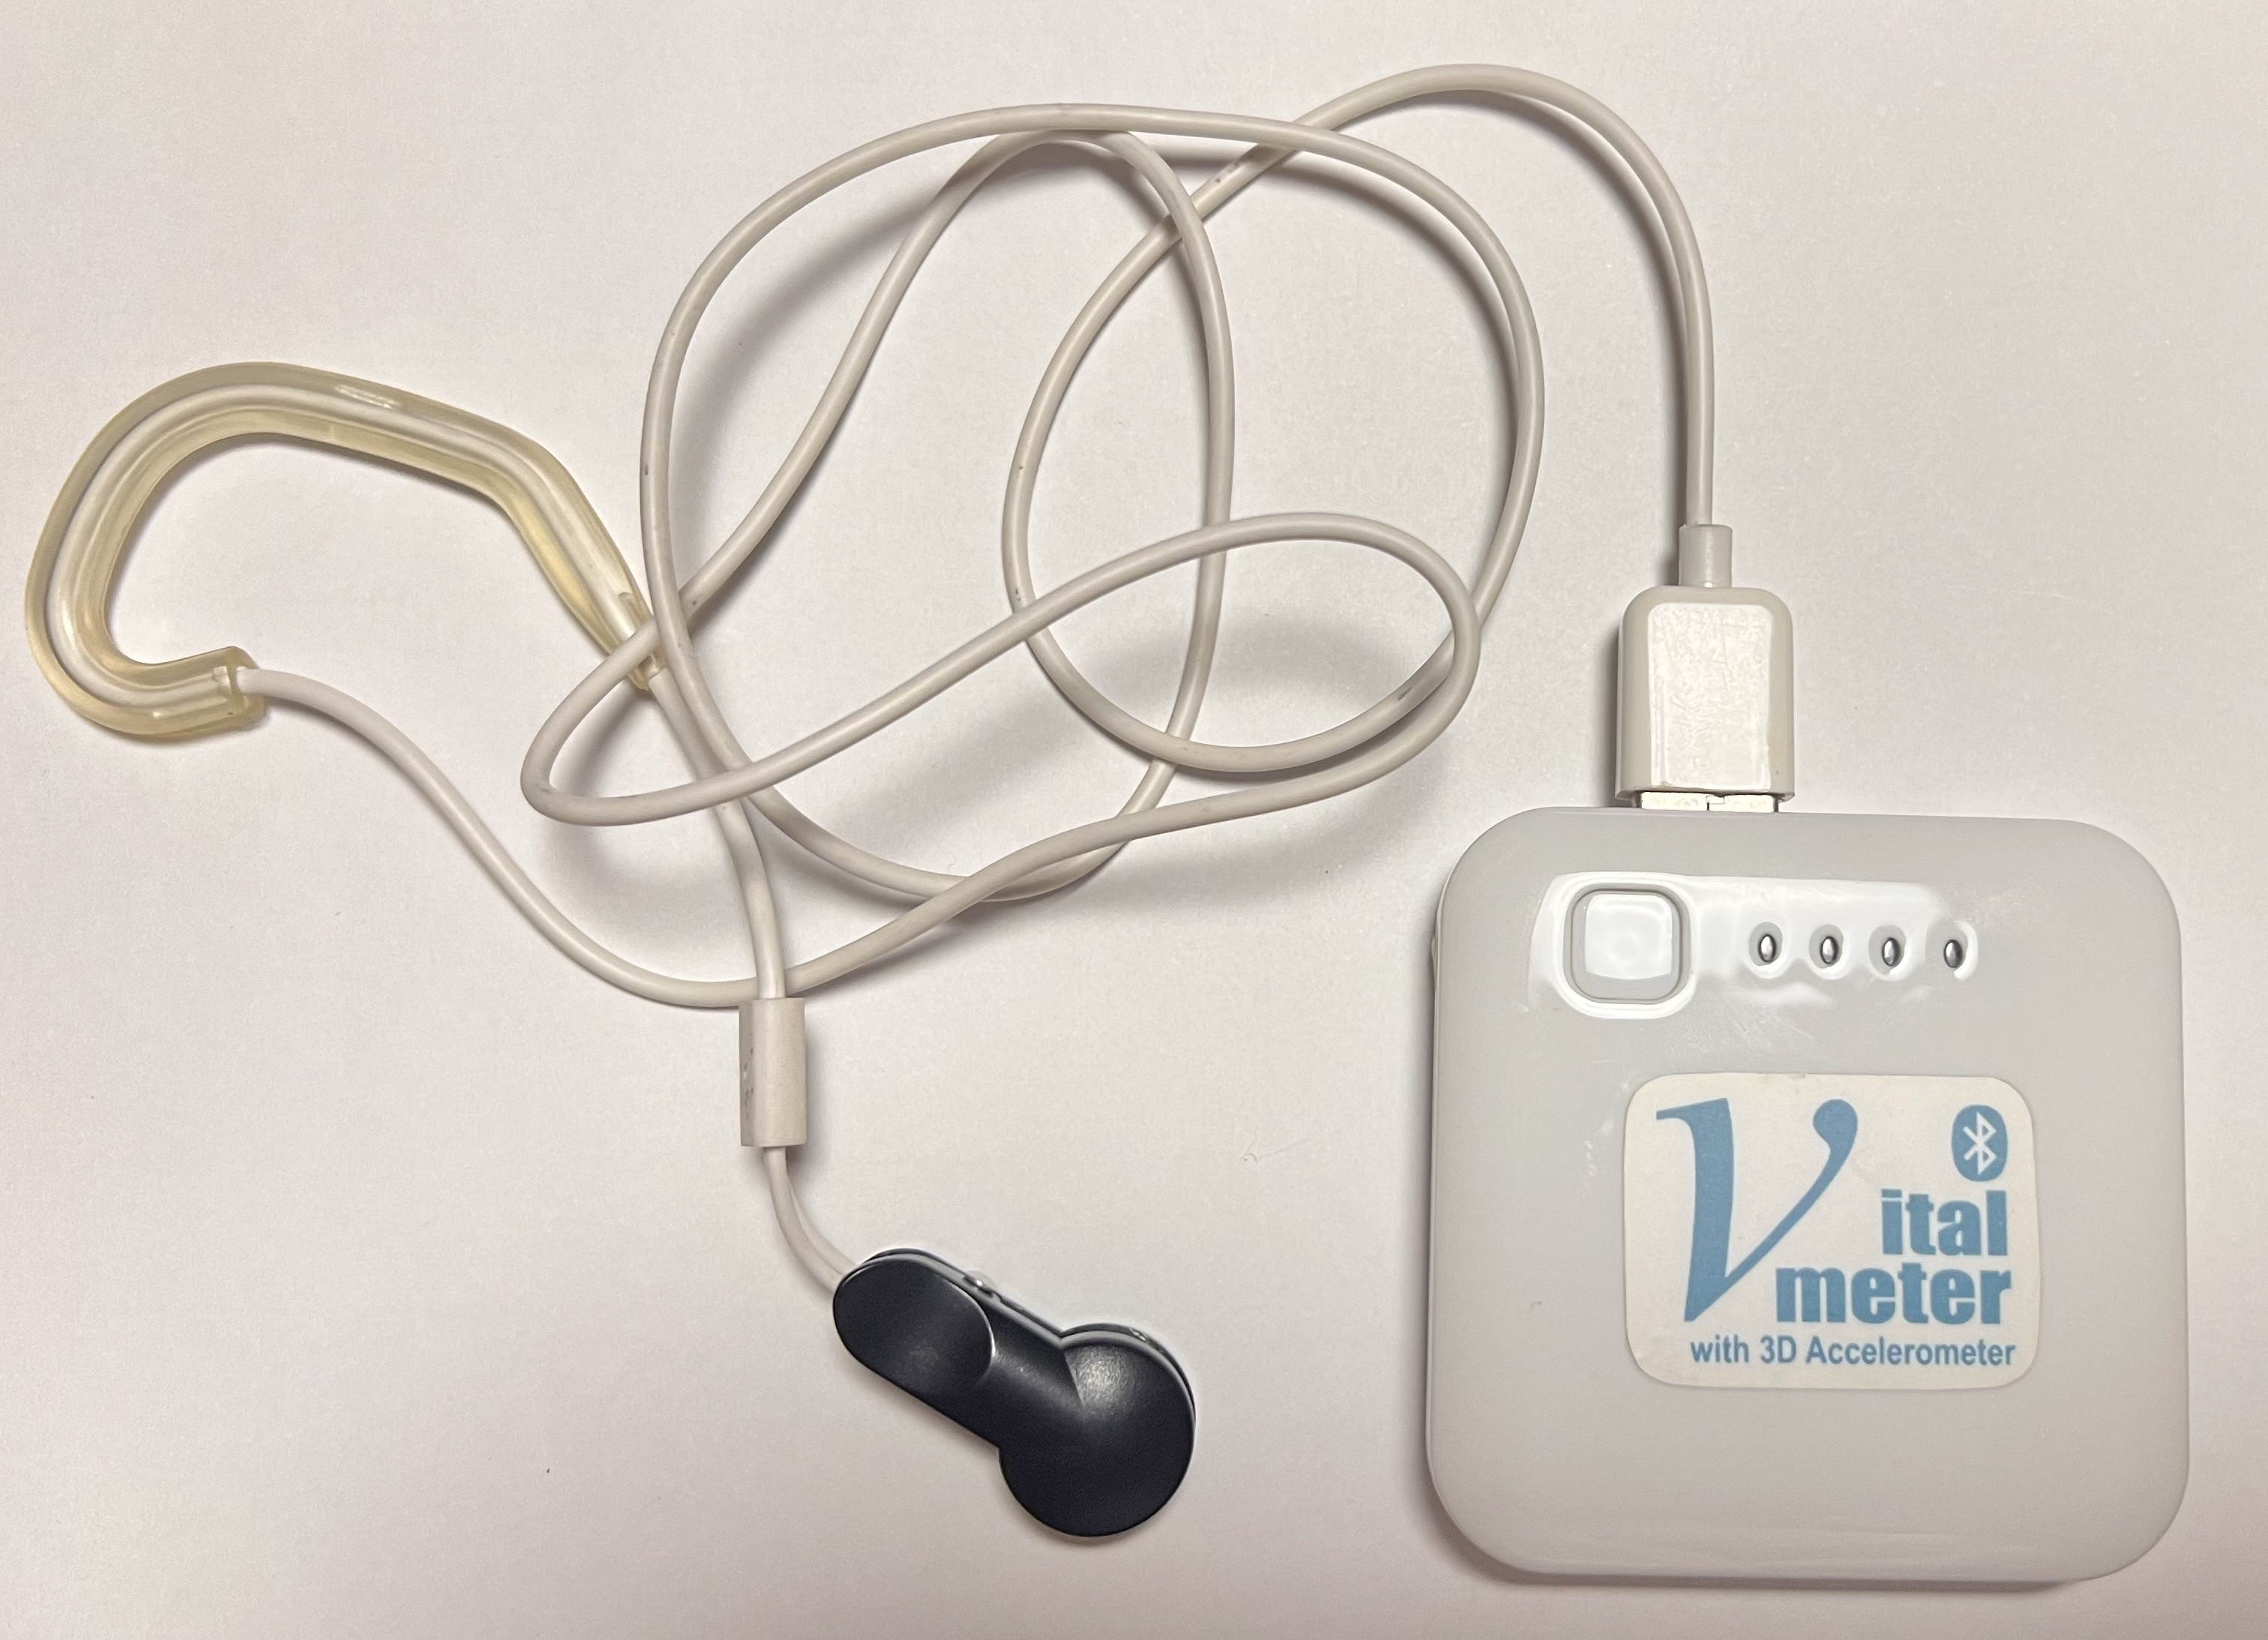
\includegraphics[width=60mm]{img/device1.jpg}
    \end{center}
    \caption{耳朶用光電式容積脈波計}
    \label{fig:device1}
  \end{minipage}
\end{figure}

光電式容積脈波(PPG)から得られる容積脈波(図\ref{fig:bvpfukuinone})をBVP(Blood Volume Pulse)といい,前述のように脈拍変動(PRV)を取得することができる.ユーザビリティ評価で容積脈波を測定する際には脈拍変動を使用することが多かった.しかし,容積脈波にはそれ自体に多くの情報が含まれており,心理学系分野では脈拍変動に限らない様々な検討されている.そもそも脈拍変動は自律神経系(ANS: Autonomic Nervous System)の影響を受けており,脈拍変動ではその変化の一部を捉えることができる\cite{peper}.

\begin{figure}[htbp]
    \begin{center}
       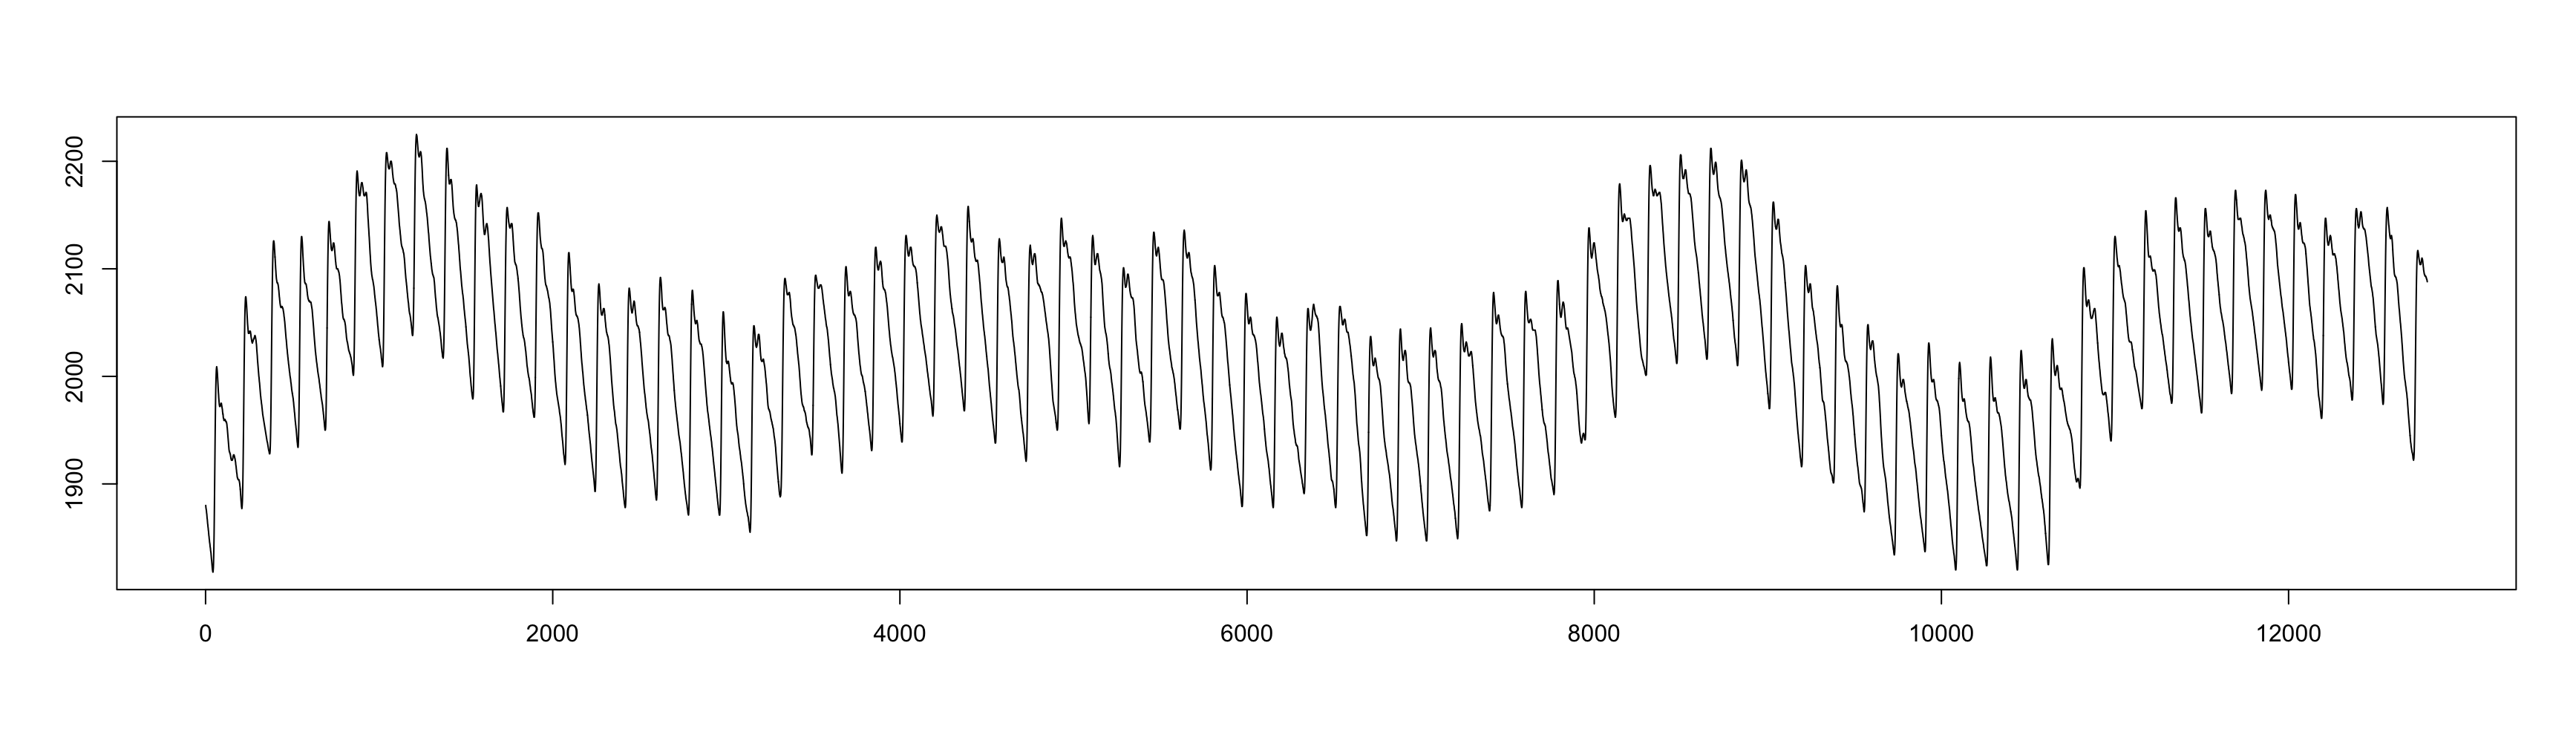
\includegraphics[width=\linewidth]{img/bvp_fukui_none.png}
    \end{center}
    \caption{PPGで取得した容積脈波}
    \label{fig:bvpfukuinone}
\end{figure}

自律神経系(ANS)はヒトの精神状態を反映していることが知られており,これを詳細に分析することでより正確にストレスを測定できる可能性がある.心拍変動(HRV)は自律神経指標として知られているが,心電図のR波とR波の間隔(RRI: R-R Interval)のことであり,RRIのゆらぎは安静時に大きくなり,ストレス時に低減する\cite{nakagawa}.RRIは容積脈波のPeek to Peekと概ね同期するため,
%引用
ここでは容積脈波から得るものもRRIと表現する.

\subsection{自律神経バランス(ANB)}

RRIのゆらぎは0.15-0.4Hzの高周波(HF: High Frequency)と0.004-0.15Hzの低周波(LF: Low Frequency)の成分に分けられ,それぞれ副交感神経活動,交感神経活動の指標として考えられている\cite{yamaguchi}.HF成分の0.15-0.4Hzは呼吸周波数(多くの人の呼吸数は秒間9-24回)であり,呼吸によるRRIの変動に対応している.この値は副交感神経が活性化すると高くなる\cite{lehrer}.LF成分は血圧変動であるメイヤー波に対応しており,交感神経と副交感神経の両方の活動を反映している.LFに対する副交感神経の影響は0.15Hz以下の深呼吸をしている間に現れる.そのためリラックスしている際は副交感神経の増大によってLFの値が高くなる\cite{trytech}.

LFとHFとの比をとることによってHF成分とLF成分のバランスを表すことができ,このバランスを自律神経バランス(ANB: Autonomic Nervous Balance)という.副交感神経はHFとLF両方に影響するためANBは交感神経の活性度と考えられる\cite{yamaguchi}.一般には数値が高いと交感神経優位,低いと副交感神経優位を表すため,高いほどストレスが高いといえる.

しかし,HF,LF,ANBで示される値はいくつかの算出方法があり,算出方法によって値が変化する.そして,自律神経以外の要因でも脈拍変動は起きるためこの値だけで判断することはできない.また,この値を計算するには3分から5分程度の計測が推奨されており\cite{nakagawa},ユーザビリティ評価での活用には制約がある.本論文ではANBを次のように定義する.

\begin{equation}
ANB= \frac{LF}{HF} 
\end{equation}

HRVを使ったユーザビリティ評価に関する研究は多いが,ANBに言及している論文は少ない\cite{lei2020}\cite{wollmann}.理由としてHRの測定に比べANBの分析はシステムの精度や専門性の高さから利用へのハードルが高い割にANBの優位性が十分に説明されていないことが想定される.よって,ANBと他指標の比較検討を行い有用性を検証する必要がある.

\subsection{最大リヤプノフ指数(LLE)}

最大リヤプノフ指数(LLE: Largest Lyapunov Exponent),カオティック\footnote{カオス(混沌)とも言い,パワー・スペクトルがいくつかの鋭いピークを持ちながらも,それとは別に連続的成分をある幅にわたって持つときこれをカオティックな運動と呼ぶ\cite{berje}}な情報である脈波変動(BVP)について計算するとそのゆらぎの度合いを示す指標となる\cite{oyama2012}.な自律神経バランス(ANB)は長年にわたって研究されており心理学系の研究等で実績があるものの,周波数領域の解析であるため3分以上の脈波計測データの使用が推奨されるように短時間での計測が難しい.本研究では一時的UX\cite{uxwhitepaper}の変化を捉えようとしており,この制約が障害になる可能性がある.そこで,時間領域で解析を行うLLEに着目した.

\begin{figure}[htbp]
    \begin{center}
       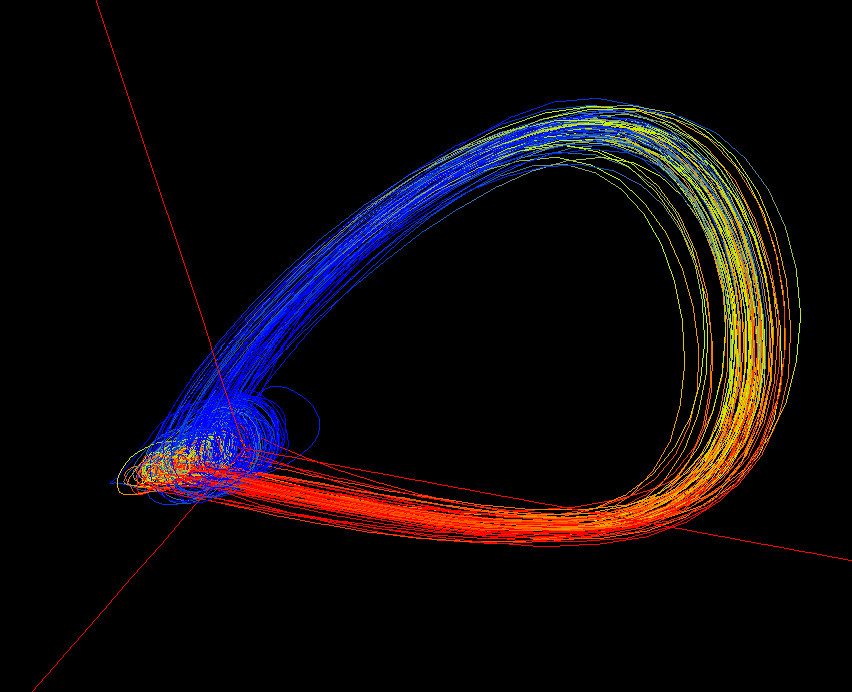
\includegraphics[width=60mm]{img/atr_fukui_none.png}
    \end{center}
    \caption{図\ref{fig:bvpfukuinone}の脈波から再構成したアトラクタ}
    \label{fig:atrfukuinone}
\end{figure}

リヤプノフ指数は,トラジェクトリー\footnote{空間中の軌跡}の分離の速さを表すことで,カオティックな流れの時間発展の追跡を容易にすることができる\cite{berje}.例えば脈波のトラジェクトリーは図\ref{fig:atrfukuinone}のようになる.実験データにおいては時間成分が含まれるため,期間内のリヤプノフ指数の最大値であるLLEを用いる.リヤプノフ指数は実験データから次のように導出される\cite{hu}.

%引用元を変更する可能性あり.雄山さんの直接の論文を引きたい

\begin{align*}
&LE= \underset{t\rightarrow\infty}{lim} \underset{\epsilon\rightarrow 0}{lim}\frac{1}{t}log\frac{\vert \delta X_{\epsilon}(t)\vert}{\vert \epsilon\vert} \tag{2}\\ 
& \quad\ \ \delta\mathrm{X}_{\epsilon}(\mathrm{t})=\mathrm{X}(\mathrm{t})-\mathrm{X}_{\epsilon}(\mathrm{t}) \tag{3}\\ 
& \quad\ \ \ \ \ \epsilon=\mathrm{X}(0)-\mathrm{X}_{\epsilon}(0) \tag{4} 
\end{align*}


雄山らは,このLLEで脈波変動(BVP)のゆらぎを解析する手法を提案している\cite{oyama2006}.そして,その指標が不安,恐怖,安堵といった精神状態と関係があることを明らかにしている\cite{imanishi2007}.雄山は著書の中で,LLEが大きいのは肯定的には行動的で積極的な状態・否定的には不安定で危なっかしい状態であり,小さいのは変化を好まないかたくなな状態・外部適応が困難な状態と表現している\cite{oyama2012book}.

LLEによる容積脈波解析に関連する研究では,LLEが精神状態の分類のほかにもストレス度の評価や様々な疾患の診断に使用できる可能性が示唆されている.Huらの研究では,学生の4-6時間の学習時にLLEとANBの変化を測定しそれらの関連を調べた結果,ストレスを示すと考えられるLLEは低下し,ANBは変動することがわかった\cite{hu}.また,認知症の程度やパーキンソン病の有無とLLEに関連があることもわかっている\cite{oyama2006dimentia}\cite{oyama2018perkinson}.ユーザビリティに関連した分野ではタスクの判断ミスや操作ミスとLLEの関連について調べた研究\cite{imanishi2006}があるが,ユーザの集中力を調査することに主眼が置かれておりシステムのユーザビリティの調査を目的としたものではない.また,小孫は論文でLLEをUX評価に活用することを提案しているが実装には至っていない\cite{komago}.

\section{問題の所在}

上述のように,UX評価では満足性を測定することが重要である.満足性を測定しうる手法として機器を用いた生理メトリクスの測定があるが,通常の開発でそれらが測定されている例は稀である.自己申告メトリクスの補完として生理メトリクスが有効であるにもかかわらず活用が浸透していない理由として次が考えられる.

\begin{itemize}
  \item 測定機器が高価かつ大がかりであり用意することが難しい
  \item 測定機器の装着自体にストレスが伴う
  \item 測定機器の装着によって手の動きなど動作が阻害される
  \item 測定や分析に特別な知識や技術が必要
  \item 測定の精度が不十分または明瞭な結果が得られない
\end{itemize}

また,UX評価を行っている場合であっても時間相を考慮した評価はほとんど行われていない.研究としてもUXグラフ\cite{kurosu2015}のような累積的UXではなく,エピソード的UXの時間変化を分析することはあまり行われてこなかった.理由として,その結果の解釈が困難であることが想定される.

以上のことから(1)容易に測定可能で専門知識がなくても結果を解釈しやすい新たな指標の提案,(2)エピソード的UXレベルでのUX変化を記録し分析できるようにすることの2点が求められる.そこで,(1)新たな指標として容積脈波による自律神経バランス(ANB)及び最大リヤプノフ指数(LLE)を提案,(2)提案指標の変化を指標としてUX変化を記録するシステムの開発を行った.